\section{Case study: the world of 2099}\label{case-study-the-world-of-2099}

2099 is a first-person automation game on a Moon base, with a prologue on Earth and a Mars expedition camp. Its central room, the hub, served as the test bench for the route; the rest of the world was then built on the route the hub settled.

\subsection{The hub in six rounds}\label{the-hub-in-six-rounds}

The hub's structure came from a cutaway the creator picked from twenty drawn from his reference pictures (Figure 1). It was then rebuilt six times on 6 and 7 October 2026 (Table 2).

\begin{figure}
\centering
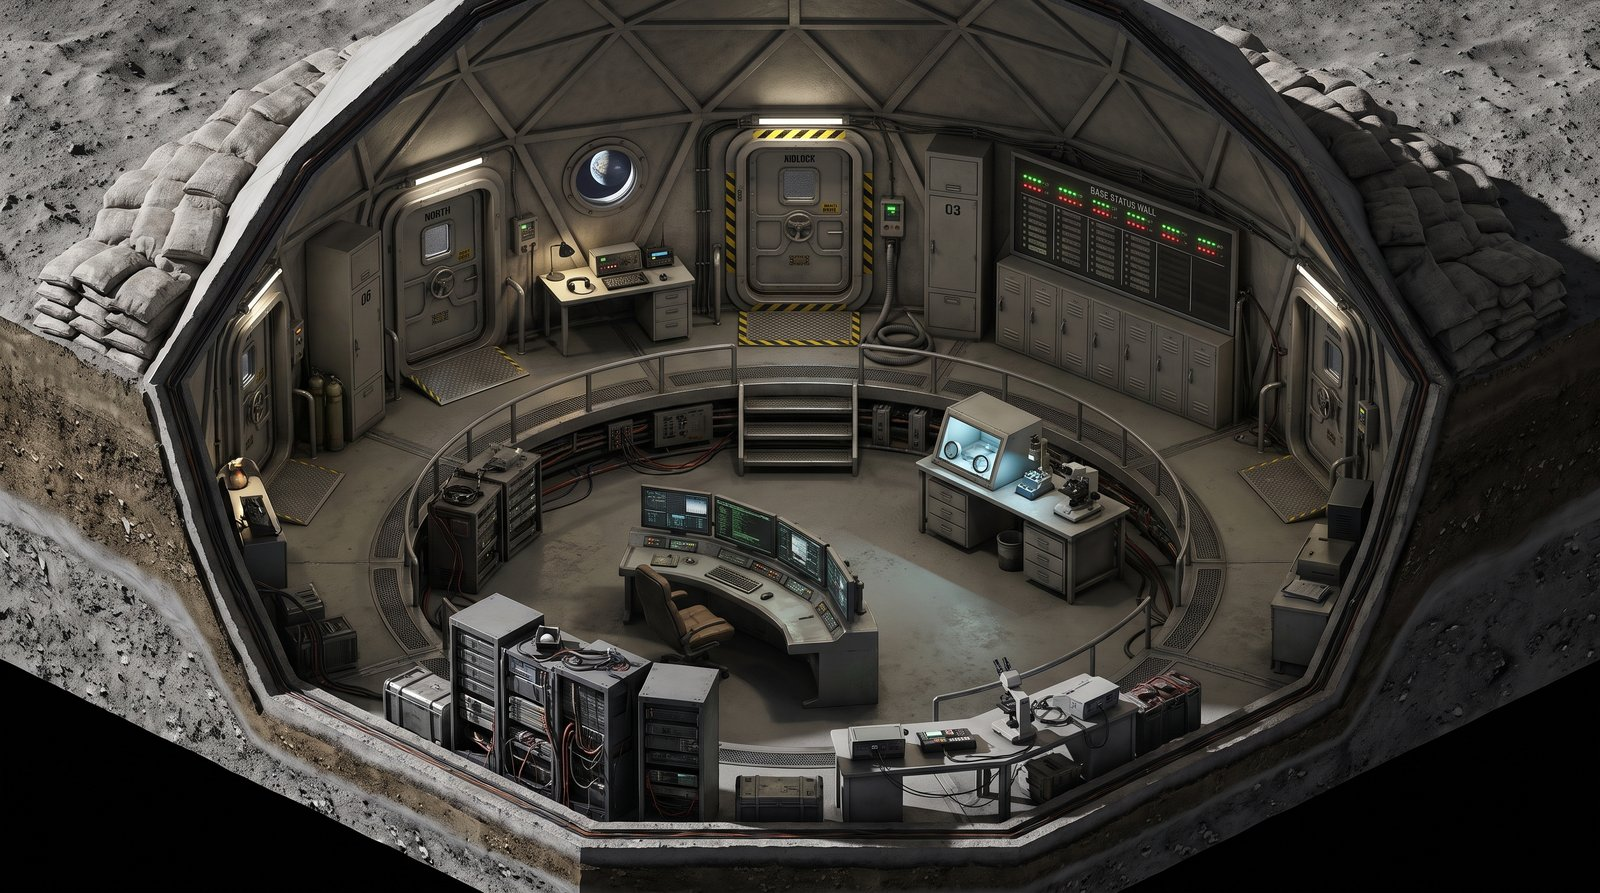
\includegraphics[width=0.8\linewidth,height=\textheight,keepaspectratio,alt={The picked concept for the hub (cutaway C12): a twelve-sided shell over a sunken pit, drawn by Nano Banana Pro from reference pictures the creator kept. It fixes the room's structure and is not shipped.}]{figures/hub-concept-c12.jpg}
\caption{The picked concept for the hub (cutaway C12): a twelve-sided shell over a sunken pit, drawn by Nano Banana Pro from reference pictures the creator kept. It fixes the room's structure and is not shipped.}
\end{figure}

\textbf{Table 2.} The hub's six rounds. Cost is rented GPU time (€) and picture calls (\$). Frame time is the mean on an RTX 5080 at night, 1600×900.

{\def\LTcaptype{none} % do not increment counter
\begin{longtable}[]{@{}
  >{\raggedright\arraybackslash}p{(\linewidth - 8\tabcolsep) * \real{0.2000}}
  >{\raggedright\arraybackslash}p{(\linewidth - 8\tabcolsep) * \real{0.2000}}
  >{\raggedright\arraybackslash}p{(\linewidth - 8\tabcolsep) * \real{0.2000}}
  >{\raggedright\arraybackslash}p{(\linewidth - 8\tabcolsep) * \real{0.2000}}
  >{\raggedright\arraybackslash}p{(\linewidth - 8\tabcolsep) * \real{0.2000}}@{}}
\toprule\noalign{}
\begin{minipage}[b]{\linewidth}\raggedright
Round
\end{minipage} & \begin{minipage}[b]{\linewidth}\raggedright
Change
\end{minipage} & \begin{minipage}[b]{\linewidth}\raggedright
Creator's verdict
\end{minipage} & \begin{minipage}[b]{\linewidth}\raggedright
Cost
\end{minipage} & \begin{minipage}[b]{\linewidth}\raggedright
Frame time
\end{minipage} \\
\midrule\noalign{}
\endhead
\bottomrule\noalign{}
\endlastfoot
1, two walls, A/B & surface library, routing by shape, room checks & blind pick for the new route (``Y looks much cleaner'') & €0.88 & 7.81 ms vs 7.53 \\
2, two walls, A/B & 71-variant library, shared texture sets, roof check & blind pick for the new route & €1.70 & 8.05 ms vs 8.24 \\
3, whole room & route end to end, 74 models & old models still loaded; labels and floor fittings wrong & €1.67 & 6.78 ms (old 9.22) \\
4, whole room & detail through the pipeline, picture colours kept & ``pretty much all of this became messy'' & €8.50, \$5.09 & 9.6 ms \\
5, eight pieces, A/B & shape only from the pipeline, library surfaces, parts check & new method preferred for door, notice board, porthole; three pieces still wrong & €0.21 & not run \\
6, whole room & round 5 everywhere, one model per object, straightness check & ``this looks amazing, I have no negative feedback'' & €3.48, \$1.07 & 5.6 ms \\
\end{longtable}
}

Three findings came out of it. First, deterministic checks found what agents missed: in round one, light escaping through walls and roof fell from 1.53 percent of 5,817 rays to zero, and colour noise within surfaces from a median of 31.1 to 3.2 percent. They did not find what only play showed: in round three 26 old models were still loaded, which led to the check that fails on any visible mesh the route did not make. Second, the split between code and pipeline was the hard decision: routing by shape lost detail (round three), keeping each picture's colours made every piece bring its own wear (round four), and the parts check with library-only surfaces and one model per object was what the creator accepted (Figure 2). Third, consistency and cost moved together: round six drew 0.45 million triangles against round four's 1.96 million, at 5.6 against 9.6 ms a frame and 187 against 487 MB on disk.

\begin{figure}
\centering
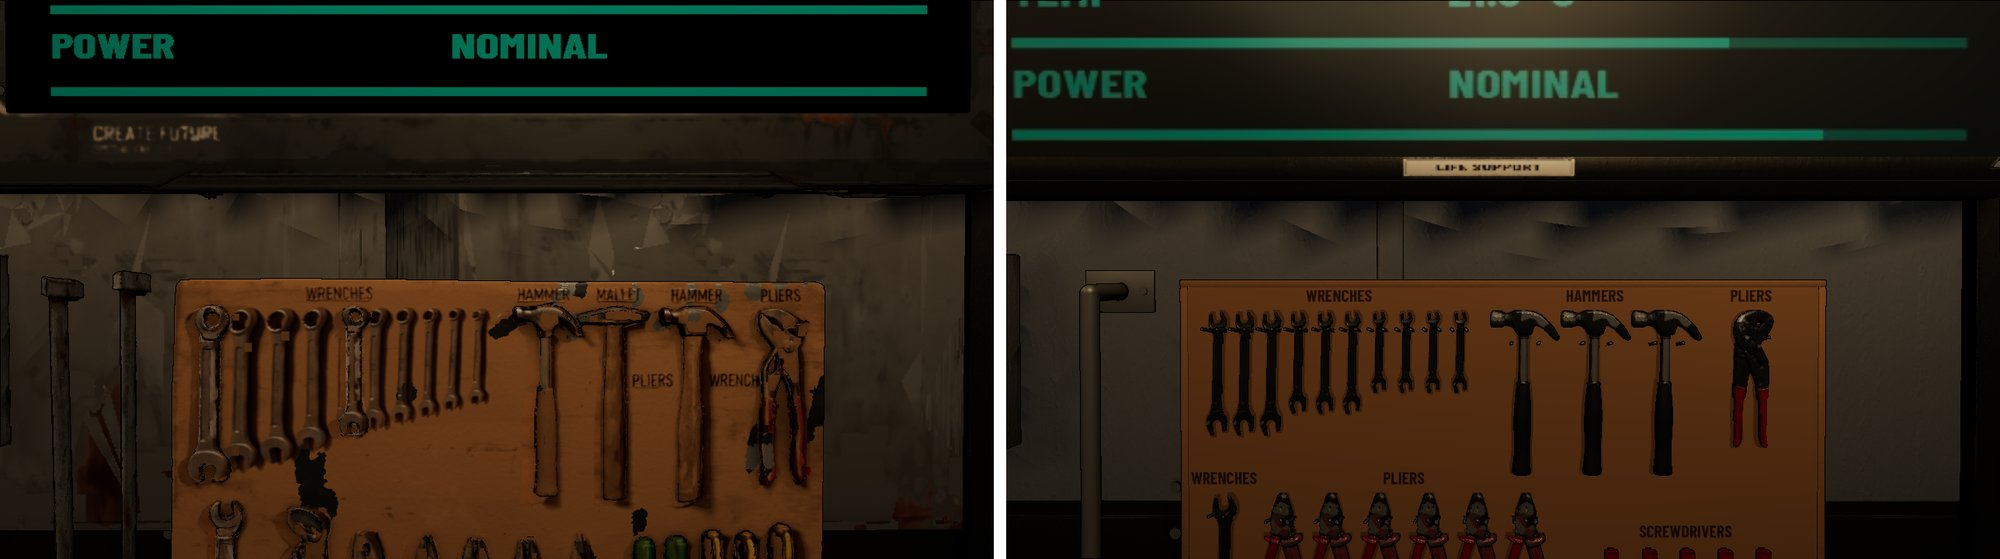
\includegraphics[width=1\linewidth,height=\textheight,keepaspectratio,alt={The hub's tool board in round four (left: one generated model with its picture's colours over library surfaces) and round six (right: a code-built board with 26 separately made tools, library surfaces only). Same camera and build.}]{figures/hub-toolboard-r4-r6.jpg}
\caption{The hub's tool board in round four (left: one generated model with its picture's colours over library surfaces) and round six (right: a code-built board with 26 separately made tools, library surfaces only). Same camera and build.}
\end{figure}

\subsection{The rest of the world}\label{the-rest-of-the-world}

After the hub was accepted, the route was run on the other places in parallel, about one agent per place, from the evening of 7 October until the game work was paused at noon on 8 October. The per-place records (21 entries) cover the planned Moon ground, the old station and the wreck, the base's lab, workshop, greenhouse, habitat, airlock and walkway tubes, the prologue's flat, stairwell, street, square and launch view, and the Mars ground, camp grounds and habitat. Together they record €46.67 of rented GPU time and \$40.72 of picture calls, as floors from the agents' notes, and 971 models: 865 code builders and 106 through the prop pipeline. Single places mostly cost a few euros, while their wall time ran to many hours, much of it waiting for machines and quotas.

The creator accepted the old station and the wreck on first sight (``it just looks great''), and preferred the planned Moon ground to a crater generated with Infinigen, in a comparison that was not blind because the two were rendered differently. The other places are built and pass their checks, but have not been reviewed by the creator in play: the game work was paused before that review, so their acceptance is open. The weaknesses were consistent across places. Code builders gave clean pieces but sparse rooms, and do not scale: each kind needs an agent to write a builder. Rooms read sparser than their concepts, which a concept shows from one side only; this gave rise to the concept-density check. Choosing surfaces by picture colour produced patchy materials. And the pace was set by daily picture quotas and GPU stock, not by compute cost. A count of faults caught per check, before and after spending, belongs here and is not given: the per-place records hold the faults as free text, which still has to be coded by hand.
